\documentclass{article}

\usepackage{graphicx}
\usepackage{amsmath}

\title{The StegChris Algorithm}
\author{Chris Nakamura}

\begin{document}

\maketitle

\section{Overview}

In the StegChris algorithm, each character in the message to be encoded is assigned to a unique 16 by 16 square of pixels. Let us assume that we are encoding the $i$th character of our message $c$ and the assigned square of pixels as $P$. Each $P$ will be assigned a starting pixel $s=(x,y)$, to be known as the starting vertex.  This is determined using a SHA256 cryptographic hash on a provided passphrase. Because there are $256$ different pixels in $P$ (recall that it is 16 by 16) $(x,y)$ will refer to a specific $p \in P$
$$t = int(hashed\_passphrase[(2*i)\%64:(2*i\%64)+2],base=16)$$
$$x = \lfloor t / 16 \rfloor$$
$$y = t \% 16$$

For simplicities sake, let us assume we are encoding the message in the red field (rather then blue, green, or alpha).  In order to make the image modifications less obvious, we will store $c$ in two values, rather then one. We will let $m$ be the average red value in $P$, excluding $(x,y)$ and $(x,y+1)$. We will define two values, at $(x,y)$ we will store $\alpha$, and at $(x,y+1)$ we will store $\beta$. 
$$\alpha = m + \lfloor \frac{c}{16}\rfloor $$
$$\beta = m + \lfloor c \% 16\rfloor$$

Because $\alpha \leq 16 \land \beta \leq 16$, this will limit the field we are editing to being at most $16$ values off the average in $P$.  This will make our changes less noticeable.

In order to decode the value, we will read $\alpha$ and $\beta$ from the image. We will again determine the start value $(x,y)$ and $(x,y+1)$, from the provided passphrase. Then the value can be decoded by the following equation.

$$c = \frac{\alpha-m}{16}+\beta-m$$

\section{Caveats}

\begin{enumerate}
	\item Note that we need to be careful about the color field that we decide to store our message in.  In the below image I have in encoded a message in both the red and the green field. As one can see, the modified green pixels are much more noticeable then the modified red ones. 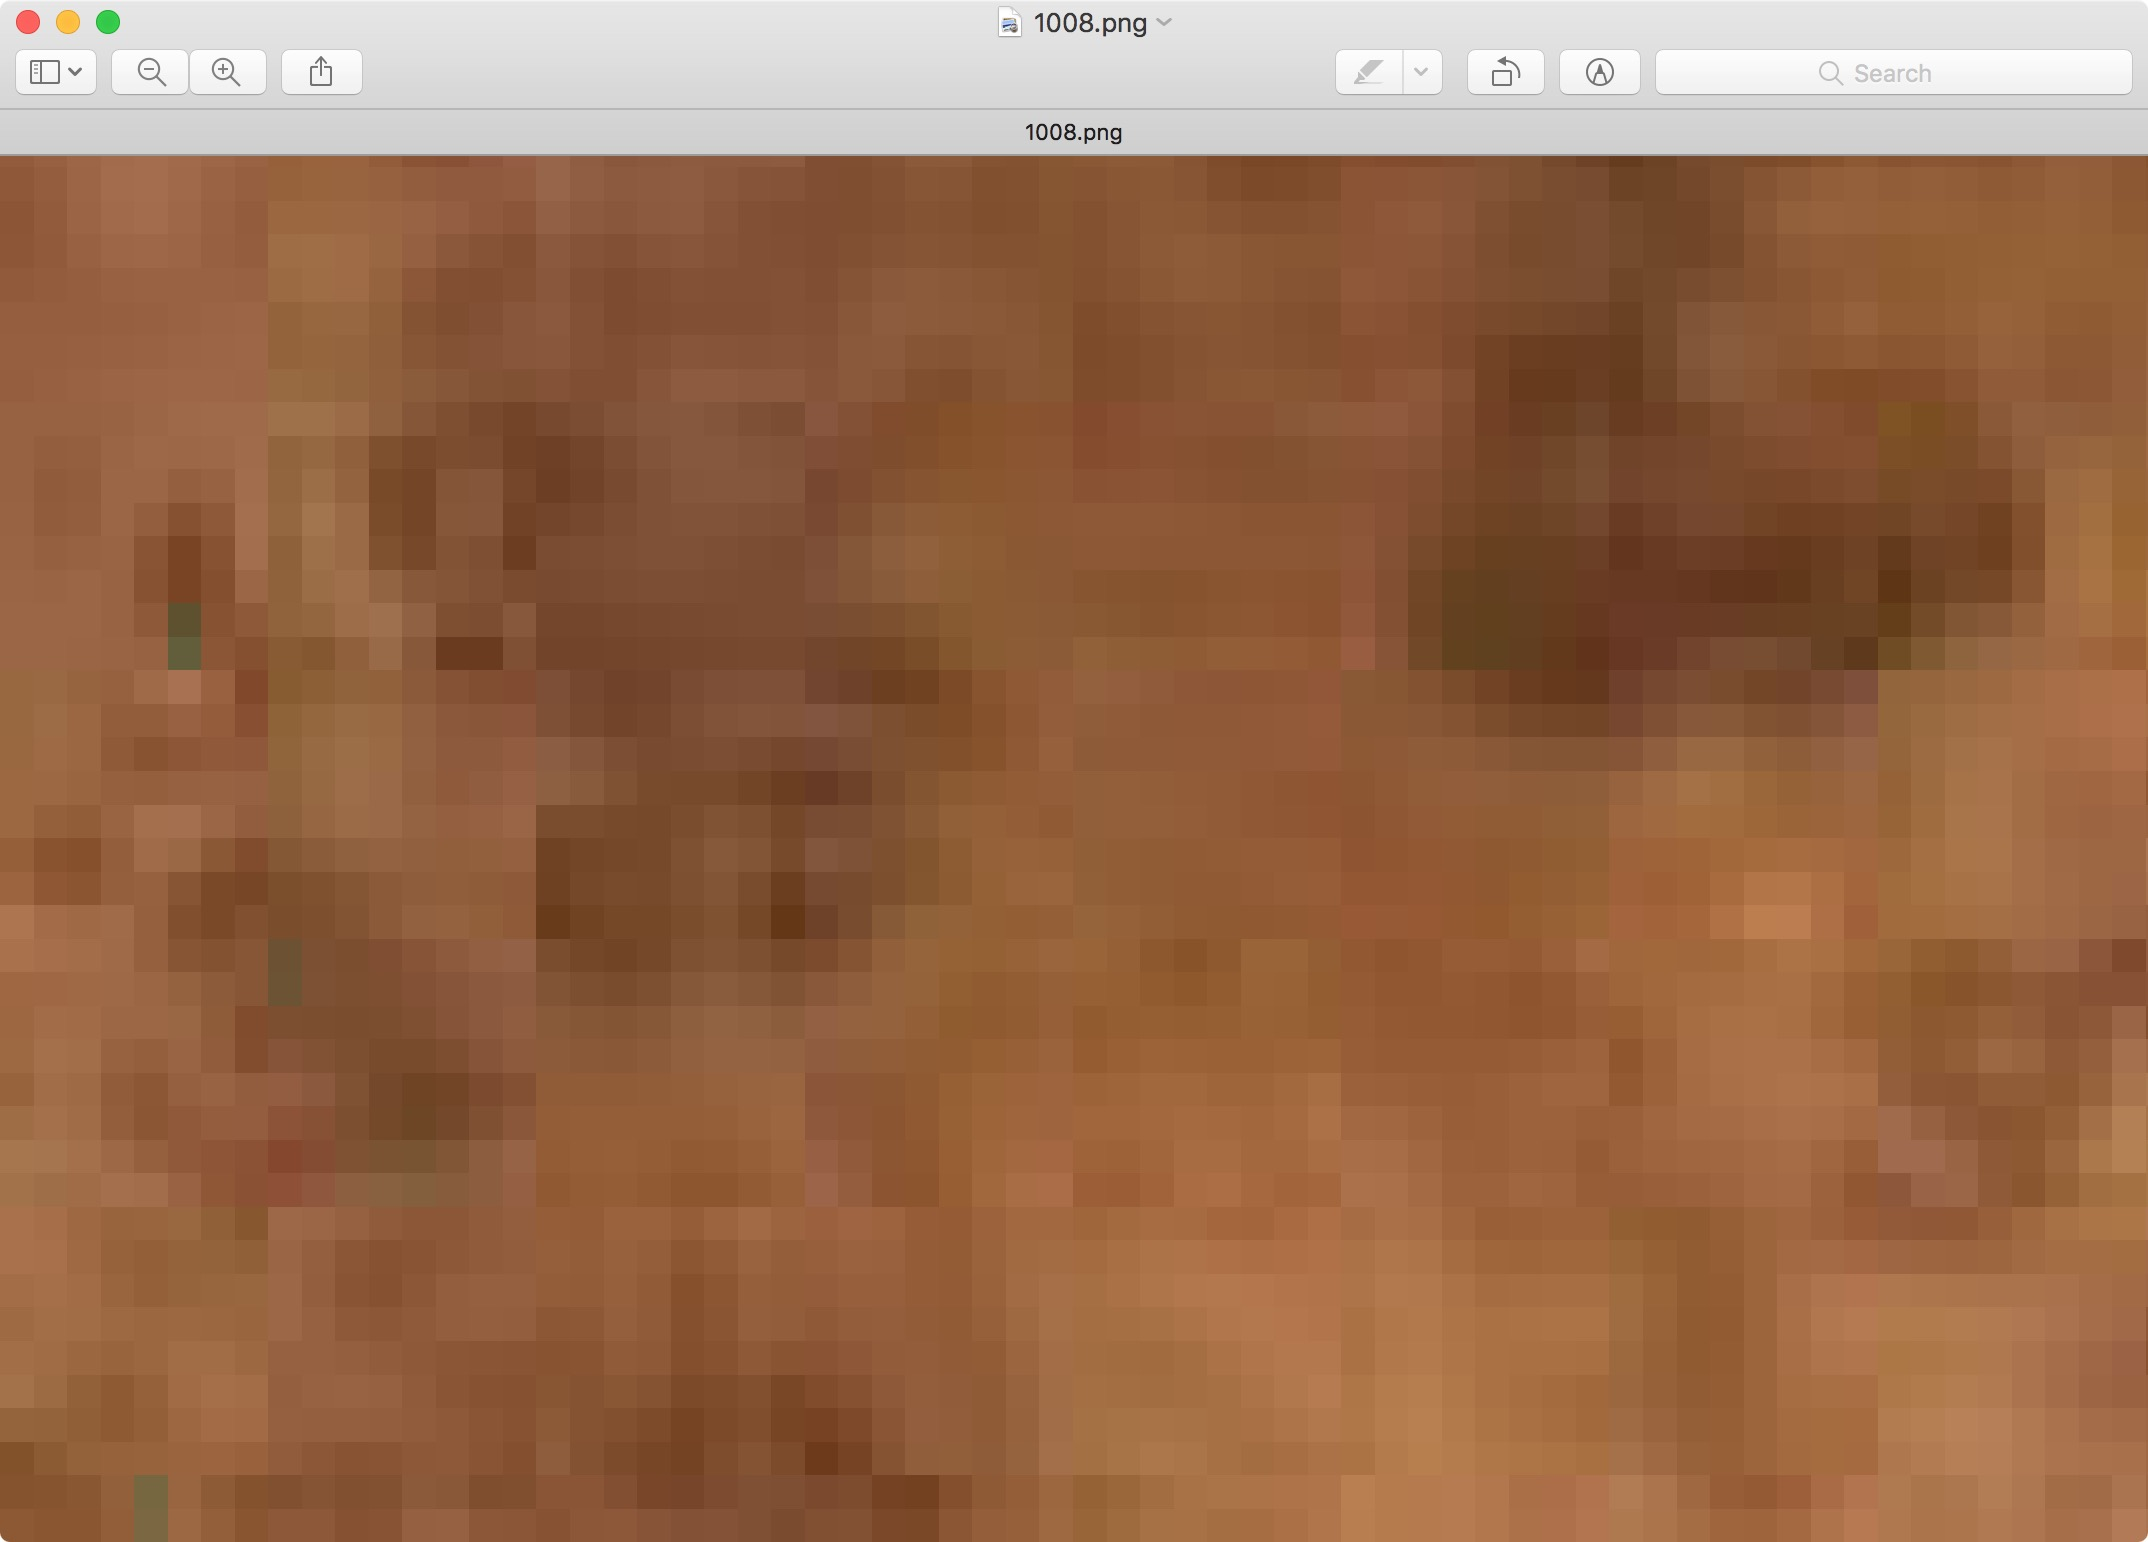
\includegraphics[width=\textwidth]
{greenvred.jpg}
	
	This is because, while $\alpha \leq 16 \land \beta \leq 16$ if $m$ is significantly small (like it is in this images), their modifications can become very noticeable.
	\item As every character requires 256 pixels to store its image, this method is very space inefficient (calculated below).
	
	$$\frac{1}{256*4 \text{ (4 bytes for r,g,b,a)}} = 0.015625 = 1.5625\%$$

	\item As a SHA256 hash is only 32 characters long. In order to encode a message longer then 32 characters, I wrapped back around to the start of the hash to determine $s$. I think the best way to fix this would be to deterministically permute the passphrase in some way, and then rehash it (but I don't know how you would go about doing this).

\end{enumerate}

\end{document}